\documentclass[aspectratio=169,10pt,t,xcolor={table}]{beamer}

% ─────────────────────────────────────────────────────────────────────────────
% EADD — JCSSE 2026 Slides v2
% Academic infographic style. Custom palette, TikZ diagrams, pgfplots charts.
% Compile: pdflatex jcsse2026_slides_v2.tex (×2 for references)
% ─────────────────────────────────────────────────────────────────────────────

\usepackage[T1]{fontenc}
\usepackage{lmodern}
\usepackage{amsmath,amssymb}
\usepackage{booktabs,array}
\usepackage{tikz}
\usetikzlibrary{arrows.meta,positioning,calc,shapes.geometric,backgrounds,fit,
                decorations.pathreplacing,decorations.pathmorphing,
                patterns,shapes.symbols,shapes.misc,matrix}
\usepackage{pgfplots}
\pgfplotsset{compat=1.18}

% ──────────────────── PALETTE ────────────────────
\definecolor{eaddDeep}{HTML}{0F3057}
\definecolor{eaddTeal}{HTML}{1B8A9C}
\definecolor{eaddCoral}{HTML}{E0625A}
\definecolor{eaddAmber}{HTML}{F4B942}
\definecolor{eaddLime}{HTML}{6FA84B}
\definecolor{eaddSlate}{HTML}{415A77}
\definecolor{eaddMist}{HTML}{F3F6FA}
\definecolor{eaddInk}{HTML}{1B2A41}

% ──────────────────── BEAMER THEME ────────────────────
\setbeamercolor{normal text}{fg=eaddInk,bg=white}
\setbeamercolor{alerted text}{fg=eaddCoral}
\setbeamercolor{example text}{fg=eaddTeal}
\setbeamercolor{frametitle}{fg=eaddDeep,bg=white}
\setbeamercolor{title}{fg=white,bg=eaddDeep}
\setbeamercolor{block title}{fg=white,bg=eaddDeep}
\setbeamercolor{block body}{fg=eaddInk,bg=eaddMist}
\setbeamercolor{itemize item}{fg=eaddTeal}
\setbeamercolor{itemize subitem}{fg=eaddCoral}
\setbeamercolor{enumerate item}{fg=eaddCoral}
\setbeamercolor{section in toc}{fg=eaddDeep}
\setbeamercolor{structure}{fg=eaddDeep}

\setbeamerfont{frametitle}{series=\bfseries,size=\Large}
\setbeamerfont{title}{series=\bfseries,size=\LARGE}
\setbeamerfont{block title}{series=\bfseries}

\setbeamertemplate{navigation symbols}{}
\setbeamertemplate{itemize item}{\raisebox{0.18ex}{\tikz\fill[eaddTeal] (0,0) rectangle (1.4ex,1.4ex);}}
\setbeamertemplate{itemize subitem}{\textcolor{eaddCoral}{\textbf{--}}}
\setbeamertemplate{enumerate item}{\textcolor{eaddCoral}{\textbf{\insertenumlabel.}}}

\setbeamertemplate{frametitle}{%
  \nointerlineskip
  \vspace{0.45em}\hspace{1.1em}%
  \begin{tikzpicture}
    \fill[eaddCoral] (0,0) rectangle (0.18,0.7);
    \node[anchor=west,inner sep=0,xshift=0.30cm,text=eaddDeep,font=\Large\bfseries] at (0,0.35) {\insertframetitle};
    \draw[eaddSlate!30,line width=0.4pt] (0.30,-0.10) -- (\paperwidth-1.6cm,-0.10);
  \end{tikzpicture}\vspace{-0.2em}%
}

\setbeamertemplate{footline}{%
  \leavevmode\hspace{1.1em}%
  \begin{tikzpicture}
    \node[anchor=east,text=eaddSlate,font=\scriptsize,inner sep=0pt]
      at (\paperwidth-2.3cm,0.55) {EADD \textbar{} JCSSE 2026 \textbar{} \insertframenumber/\inserttotalframenumber};
    \fill[eaddMist] (0,0) rectangle (\paperwidth-2.2cm,0.18);
    \pgfmathsetmacro{\progfrac}{\insertframenumber/\inserttotalframenumber}
    \fill[eaddTeal] (0,0) rectangle ({(\paperwidth-2.2cm)*\progfrac},0.18);
  \end{tikzpicture}\vspace{0.20em}%
}

% ──────────────────── HELPERS ────────────────────
\newcommand{\statTile}[3]{%
  \begin{tikzpicture}
    \node[draw=#3,line width=1.2pt,rounded corners=4pt,fill=#3!8,
          minimum width=3.05cm,minimum height=1.85cm,inner sep=4pt] (b) {};
    \node[anchor=center,text=#3,font=\fontsize{22}{24}\bfseries] at ([yshift=4pt]b.center) {#1};
    \node[anchor=center,text=eaddSlate,font=\scriptsize,align=center] at ([yshift=-14pt]b.center) {#2};
  \end{tikzpicture}%
}

\newcommand{\chip}[2]{%
  \tikz[baseline=(x.base)]{\node[fill=#1!15,draw=#1,line width=0.6pt,
    rounded corners=2pt,inner xsep=4pt,inner ysep=1.2pt,font=\scriptsize\bfseries,
    text=#1] (x) {#2};}}

\newcommand{\sectionDivider}[2]{%
  \begin{frame}[plain,noframenumbering]
    \begin{tikzpicture}[remember picture,overlay]
      \fill[eaddDeep] (current page.south west) rectangle (current page.north east);
      \node[anchor=west,text=eaddCoral,font=\fontsize{120}{120}\bfseries,opacity=0.35]
        at ([xshift=1cm]current page.west) {#1};
      \node[anchor=west,text=white,font=\Huge\bfseries]
        at ([xshift=5cm,yshift=0.6cm]current page.west) {#2};
      \node[anchor=west,text=eaddAmber]
        at ([xshift=5cm,yshift=-0.4cm]current page.west) {\rule{1.2cm}{2pt}};
      \node[anchor=south west,text=white!60,font=\scriptsize]
        at ([xshift=1cm,yshift=1cm]current page.south west) {EADD \textbar{} Enhanced Adversarial Drift Detection};
    \end{tikzpicture}
  \end{frame}
}

% ──────────────────── METADATA ────────────────────
\title[EADD for MLOps Feature Monitoring]{Enhanced Adversarial Drift Detection \\
       \large for MLOps Feature Monitoring}
\author[Begum et al.]{Nusrat Begum, Phaphontee Yamchote, Chainarong Amornbunchornvej, Thanapon Noraset}
\institute{Mahidol University \textbar{} NECTEC}
\date{JCSSE 2026 \textbar{} Bangkok \textbar{} June 24--27, 2026}

\begin{document}

% ════════════════════ TITLE ════════════════════
\begin{frame}[plain,noframenumbering]
\begin{tikzpicture}[remember picture,overlay]
  \fill[eaddDeep] (current page.south west) rectangle (current page.north east);
  \fill[eaddTeal,opacity=0.55]
    (current page.north west) -- ([xshift=8cm]current page.north west)
    -- ([xshift=4cm]current page.south west) -- (current page.south west) -- cycle;
  \foreach \i in {0,1,2,3,4,5,6,7}{
    \fill[eaddAmber,opacity={0.06+0.02*\i}]
      ([xshift=-2cm-0.4*\i cm,yshift=-2cm-0.3*\i cm]current page.north east)
      circle ({1.2cm+0.4*\i cm});
  }
  \fill[eaddCoral,opacity=0.85]
    ([xshift=-3.5cm,yshift=-2.3cm]current page.north east) circle (0.30cm);

  \node[anchor=west,text=eaddAmber,font=\small\bfseries]
    at ([xshift=1.0cm,yshift=2.4cm]current page.west)
    {\rule{0.6cm}{2pt}\hspace{0.4em}STREAMING ML \textbar{} DRIFT DETECTION \textbar{} EXPLAINABLE AI};

  \node[anchor=west,text=white,font=\fontsize{26}{30}\bfseries,align=left]
    at ([xshift=1.0cm,yshift=0.9cm]current page.west)
    {Enhanced Adversarial\\Drift Detection};
  \node[anchor=west,text=eaddAmber,font=\Large\itshape,align=left]
    at ([xshift=1.0cm,yshift=-0.7cm]current page.west)
    {for MLOps Feature Monitoring};

  \node[anchor=west,text=white,font=\small,align=left]
    at ([xshift=1.0cm,yshift=-1.9cm]current page.west)
    {\textbf{Nusrat Begum}$^{1}$ \enspace Phaphontee Yamchote$^{1}$ \enspace
     Chainarong Amornbunchornvej$^{2}$ \enspace Thanapon Noraset$^{1}$};
  \node[anchor=west,text=white!75,font=\scriptsize,align=left]
    at ([xshift=1.0cm,yshift=-2.4cm]current page.west)
    {$^{1}$Faculty of ICT, Mahidol University \quad $^{2}$NECTEC, NSTDA, Thailand};

  \fill[eaddAmber] ([yshift=1.5cm]current page.south west)
    rectangle ([yshift=1.42cm]current page.south east);
  \node[anchor=south west,text=white,font=\small\bfseries]
    at ([xshift=1.6cm,yshift=0.5cm]current page.south west)
    {JCSSE 2026};
  \node[anchor=south west,text=white!75,font=\small]
    at ([xshift=3.4cm,yshift=0.5cm]current page.south west)
    {Bangkok, Thailand \textbar{} June 24--27, 2026};
\end{tikzpicture}
\end{frame}

% ════════════════════ ROADMAP ════════════════════
\begin{frame}{Roadmap}
\vspace{0.2em}
\centering
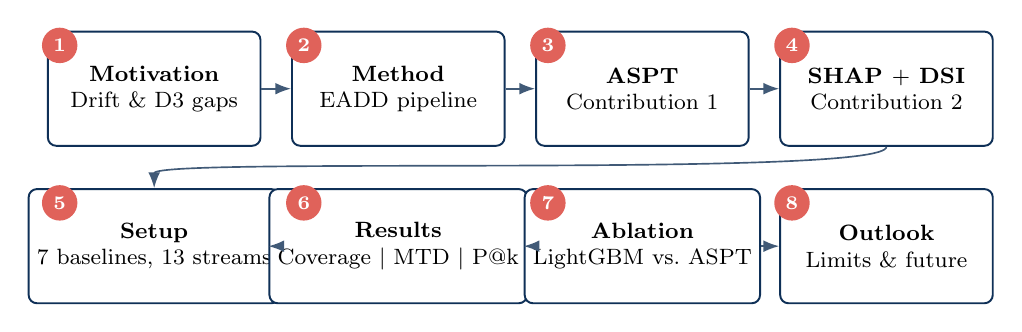
\begin{tikzpicture}[font=\footnotesize,
    stepbox/.style={draw=eaddDeep,fill=white,line width=0.7pt,rounded corners=3pt,
                  minimum width=2.7cm,minimum height=1.45cm,align=center,inner sep=3pt},
    num/.style={circle,fill=eaddCoral,text=white,font=\scriptsize\bfseries,
                inner sep=0pt,minimum size=4.5mm},
    arr/.style={-{Latex[length=2mm]},eaddSlate,line width=0.6pt}]
  \node[stepbox] (s1) at (0,0)    {\textbf{Motivation}\\Drift \& D3 gaps};
  \node[stepbox] (s2) at (3.1,0)  {\textbf{Method}\\EADD pipeline};
  \node[stepbox] (s3) at (6.2,0)  {\textbf{ASPT}\\Contribution 1};
  \node[stepbox] (s4) at (9.3,0)  {\textbf{SHAP $+$ DSI}\\Contribution 2};
  \node[stepbox] (s5) at (0,-2)   {\textbf{Setup}\\7 baselines, 13 streams};
  \node[stepbox] (s6) at (3.1,-2) {\textbf{Results}\\Coverage \textbar{} MTD \textbar{} P@k};
  \node[stepbox] (s7) at (6.2,-2) {\textbf{Ablation}\\LightGBM vs.\ ASPT};
  \node[stepbox] (s8) at (9.3,-2) {\textbf{Outlook}\\Limits \& future};
  \foreach \i/\n in {s1/1,s2/2,s3/3,s4/4,s5/5,s6/6,s7/7,s8/8}
    \node[num] at ([xshift=-1.2cm,yshift=0.55cm]\i.center) {\n};
  \draw[arr] (s1) -- (s2); \draw[arr] (s2) -- (s3); \draw[arr] (s3) -- (s4);
  \draw[arr] (s4.south) .. controls ([yshift=-0.4cm]s4.south) and ([yshift=0.4cm]s5.north) .. (s5.north);
  \draw[arr] (s5) -- (s6); \draw[arr] (s6) -- (s7); \draw[arr] (s7) -- (s8);
\end{tikzpicture}

\vspace{0.8em}
\centering\small\itshape\color{eaddSlate}
EADD answers \textcolor{eaddCoral}{\textbf{whether}}, \textcolor{eaddCoral}{\textbf{when}},
\textcolor{eaddCoral}{\textbf{which}}, and \textcolor{eaddCoral}{\textbf{how severe}} in one pipeline.
\end{frame}

% ════════════════════ SECTION 1 ════════════════════
\sectionDivider{01}{The Problem}

\begin{frame}{Production ML Models Fail Silently}
\begin{columns}[T,onlytextwidth]
\column{0.55\textwidth}
\centering
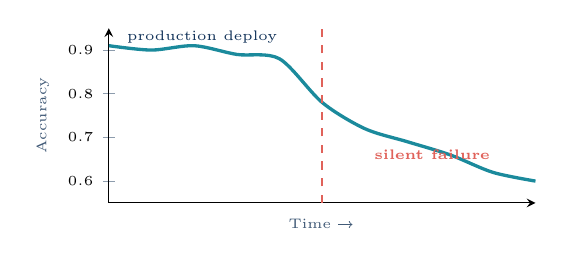
\begin{tikzpicture}[font=\scriptsize]
  \begin{axis}[
    width=7.0cm,height=3.8cm,
    axis lines=left,
    xlabel={Time \textrightarrow{}},
    ylabel={Accuracy},
    ymin=0.55,ymax=0.95,xmin=0,xmax=10,
    xtick=\empty,
    ytick={0.6,0.7,0.8,0.9},
    yticklabel style={font=\tiny},
    xlabel style={font=\tiny,text=eaddSlate},
    ylabel style={font=\tiny,text=eaddSlate},
    tick style={eaddSlate!60},
    every axis line/.style={eaddSlate!60},
  ]
    \addplot[eaddTeal,line width=1.2pt,smooth] coordinates
      {(0,0.91)(1,0.90)(2,0.91)(3,0.89)(4,0.88)(5,0.78)(6,0.72)(7,0.69)(8,0.66)(9,0.62)(10,0.60)};
    \draw[eaddCoral,dashed,line width=0.8pt] (axis cs:5,0.55) -- (axis cs:5,0.95);
    \node[text=eaddCoral,font=\tiny\bfseries,anchor=south] at (axis cs:5,0.95) {drift onset};
    \node[text=eaddDeep,font=\tiny,anchor=west] at (axis cs:0.2,0.93) {production deploy};
    \node[text=eaddCoral,font=\tiny\bfseries,anchor=west] at (axis cs:6,0.66) {silent failure};
  \end{axis}
\end{tikzpicture}

\smallskip
{\footnotesize\textbf{Distribution drift} silently degrades models.
Existing detectors raise a binary alarm; practitioners need more:}

\smallskip
\centering
\chip{eaddCoral}{Which features?}\;
\chip{eaddCoral}{How severe?}\;
\chip{eaddCoral}{Real or noise?}

\column{0.45\textwidth}
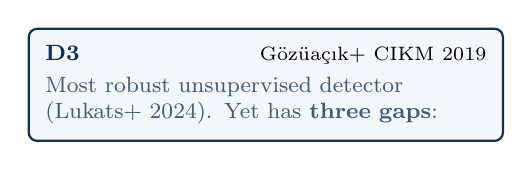
\begin{tikzpicture}
  \node[draw=eaddDeep,fill=eaddMist,line width=0.8pt,rounded corners=3pt,
        inner sep=6pt,text width=5.6cm,align=left,font=\footnotesize] (card) {%
    \textbf{\color{eaddDeep}D3} \hfill {\scriptsize Gözüaçık+ CIKM 2019}\\[2pt]
    {\color{eaddSlate}Most robust unsupervised detector (Lukats+ 2024).
    Yet has \textbf{three gaps}:}
  };
\end{tikzpicture}

\vspace{0.3em}
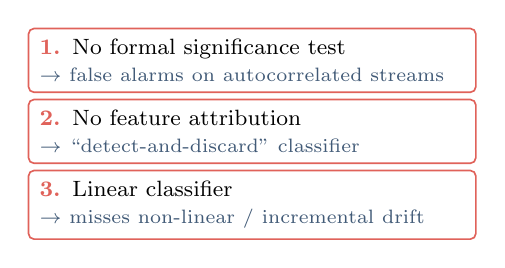
\begin{tikzpicture}[font=\footnotesize,
   gap/.style={draw=eaddCoral,fill=white,line width=0.6pt,rounded corners=2pt,
               text width=5.4cm,align=left,inner sep=4pt}]
  \node[gap] (g1) {\textcolor{eaddCoral}{\textbf{1.}} No formal significance test\\
    \scriptsize\color{eaddSlate}$\to$ false alarms on autocorrelated streams};
  \node[gap,below=2pt of g1] (g2) {\textcolor{eaddCoral}{\textbf{2.}} No feature attribution\\
    \scriptsize\color{eaddSlate}$\to$ ``detect-and-discard'' classifier};
  \node[gap,below=2pt of g2] (g3) {\textcolor{eaddCoral}{\textbf{3.}} Linear classifier\\
    \scriptsize\color{eaddSlate}$\to$ misses non-linear / incremental drift};
\end{tikzpicture}
\end{columns}
\end{frame}

\begin{frame}{Research Gap \textbar{} Capability Matrix}
\vspace{0.2em}
\centering

\begin{tikzpicture}[font=\footnotesize,
    qcard/.style={draw,line width=1pt,rounded corners=4pt,
                  minimum width=3.5cm,minimum height=1.3cm,align=center,
                  inner sep=4pt}]
  \node[qcard,draw=eaddDeep,fill=eaddDeep!8]   (q1) at (-5.4,0)
    {\textbf{\color{eaddDeep}WHETHER?}\\[2pt]\scriptsize\color{eaddSlate}Binary drift alarm};
  \node[qcard,draw=eaddCoral,fill=eaddCoral!8] (q2) at (0,0)
    {\textbf{\color{eaddCoral}WHICH?}\\[2pt]\scriptsize\color{eaddSlate}Feature attribution};
  \node[qcard,draw=eaddAmber!85!black,fill=eaddAmber!18] (q3) at (5.4,0)
    {\textbf{\color{eaddAmber!70!black}HOW SEVERE?}\\[2pt]\scriptsize\color{eaddSlate}Severity quantification};
\end{tikzpicture}

\vspace{0.6em}
\centering
\renewcommand{\arraystretch}{1.25}
\setlength{\tabcolsep}{8pt}
{\footnotesize
\begin{tabular}{@{}>{\raggedright\arraybackslash}p{3.6cm} c c c c@{}}
\toprule
\rowcolor{eaddDeep!90}
\textcolor{white}{\textbf{Approach}} & \textcolor{white}{\textbf{Whether}} &
\textcolor{white}{\textbf{Which}}    & \textcolor{white}{\textbf{Severity}}  &
\textcolor{white}{\textbf{Streaming}} \\
\midrule
DDM / EDDM          & {\color{eaddLime}$\checkmark$} & {\color{eaddCoral}$\times$} & {\color{eaddCoral}$\times$} & {\color{eaddLime}$\checkmark$} \\
KS / KSWIN          & {\color{eaddLime}$\checkmark$} & {\color{eaddAmber!70!black}$\sim$} & {\color{eaddCoral}$\times$} & {\color{eaddLime}$\checkmark$} \\
D3                  & {\color{eaddLime}$\checkmark$} & {\color{eaddCoral}$\times$} & {\color{eaddCoral}$\times$} & {\color{eaddLime}$\checkmark$} \\
Vertex AI / Clarify & {\color{eaddLime}$\checkmark$} & {\color{eaddLime}$\checkmark$} & {\color{eaddAmber!70!black}$\sim$} & {\color{eaddCoral}$\times$} \\
TRIPODD / HDPD      & {\color{eaddLime}$\checkmark$} & {\color{eaddLime}$\checkmark$} & {\color{eaddCoral}$\times$} & {\color{eaddCoral}$\times$} \\
\midrule
\rowcolor{eaddTeal!90}
\textcolor{white}{\textbf{EADD (this work)}} &
\textcolor{white}{$\checkmark$} & \textcolor{white}{$\checkmark$} &
\textcolor{white}{$\checkmark$} & \textcolor{white}{$\checkmark$} \\
\bottomrule
\end{tabular}}
\end{frame}

\begin{frame}{Three Contributions at a Glance}
\vspace{0.3em}
\centering
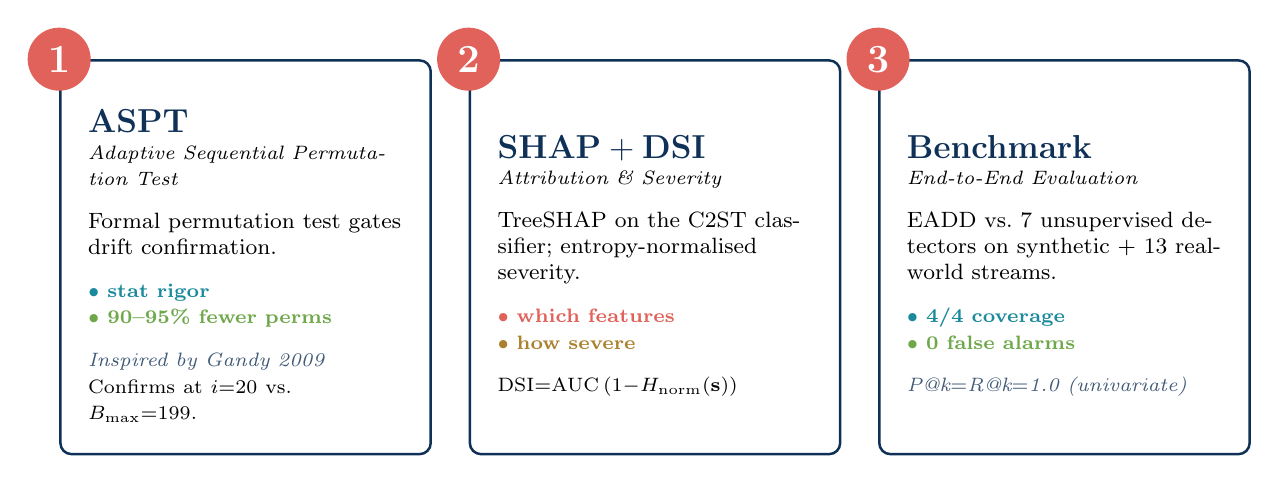
\begin{tikzpicture}[font=\footnotesize,
    card/.style={draw=eaddDeep,line width=0.9pt,rounded corners=4pt,
                 fill=white,minimum width=4.5cm,minimum height=5.0cm,
                 inner sep=10pt,align=left,text width=4.0cm,anchor=center},
    badge/.style={circle,fill=eaddCoral,text=white,font=\Large\bfseries,
                  inner sep=0pt,minimum size=8mm}]

  \node[card] (c1) at (-5.2,0) {%
    \vspace{0.6em}\\
    \textbf{\color{eaddDeep}\large ASPT}\\
    {\scriptsize\itshape Adaptive Sequential Permutation Test}\\[6pt]
    Formal permutation test gates drift confirmation.\\[6pt]
    {\scriptsize\color{eaddTeal}\textbf{$\bullet$ stat rigor}}\\
    {\scriptsize\color{eaddLime}\textbf{$\bullet$ 90--95\% fewer perms}}\\[6pt]
    {\scriptsize\color{eaddSlate}\itshape Inspired by Gandy 2009}\\
    {\scriptsize Confirms at $i{=}20$ vs.\ $B_{\max}{=}199$.}};
  \node[card] (c2) at (0,0) {%
    \vspace{0.6em}\\
    \textbf{\color{eaddDeep}\large SHAP $+$ DSI}\\
    {\scriptsize\itshape Attribution \& Severity}\\[6pt]
    TreeSHAP on the C2ST classifier; entropy-normalised severity.\\[6pt]
    {\scriptsize\color{eaddCoral}\textbf{$\bullet$ which features}}\\
    {\scriptsize\color{eaddAmber!70!black}\textbf{$\bullet$ how severe}}\\[6pt]
    {\scriptsize $\mathrm{DSI}{=}\mathrm{AUC}\,(1{-}H_{\mathrm{norm}}(\mathbf{s}))$}};
  \node[card] (c3) at (5.2,0) {%
    \vspace{0.6em}\\
    \textbf{\color{eaddDeep}\large Benchmark}\\
    {\scriptsize\itshape End-to-End Evaluation}\\[6pt]
    EADD vs.\ 7 unsupervised detectors on synthetic $+$ 13 real-world streams.\\[6pt]
    {\scriptsize\color{eaddTeal}\textbf{$\bullet$ 4/4 coverage}}\\
    {\scriptsize\color{eaddLime}\textbf{$\bullet$ 0 false alarms}}\\[6pt]
    {\scriptsize\color{eaddSlate}\itshape P@k$=$R@k$=$1.0 (univariate)}};

  \node[badge] at (c1.north west) {1};
  \node[badge] at (c2.north west) {2};
  \node[badge] at (c3.north west) {3};
\end{tikzpicture}
\end{frame}

% ════════════════════ SECTION 2 ════════════════════
\sectionDivider{02}{The EADD Pipeline}

\begin{frame}{End-to-End Detection Pipeline}
\vspace{-0.3em}
\centering
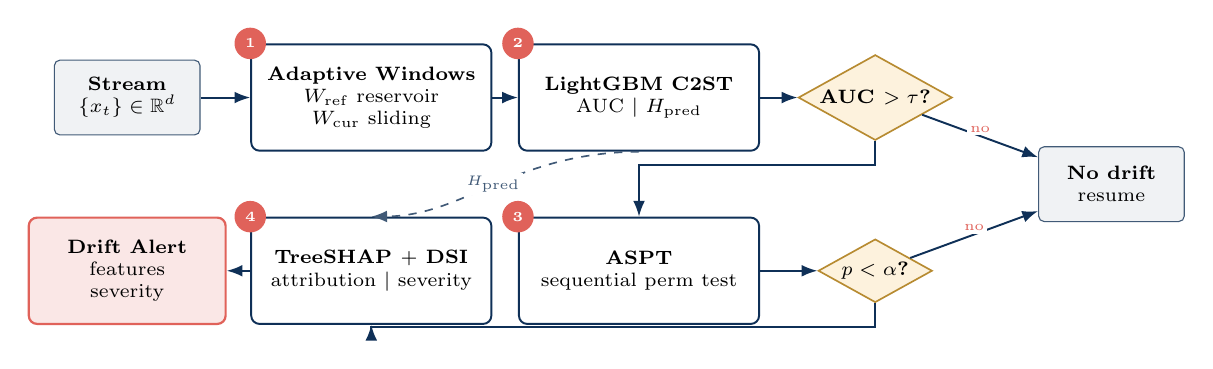
\begin{tikzpicture}[font=\scriptsize,
    proc/.style={draw=eaddDeep,fill=white,line width=0.7pt,rounded corners=3pt,
                 minimum width=3.05cm,minimum height=1.35cm,align=center,inner sep=3pt},
    dec/.style={diamond,draw=eaddAmber!75!black,fill=eaddAmber!18,line width=0.6pt,
                aspect=1.8,align=center,inner sep=1pt,font=\scriptsize\bfseries},
    term/.style={draw=eaddSlate,fill=eaddSlate!8,rounded corners=2pt,align=center,
                  minimum width=1.85cm,minimum height=0.95cm},
    alert/.style={draw=eaddCoral,fill=eaddCoral!15,line width=0.8pt,rounded corners=3pt,
                  align=center,minimum width=2.5cm,minimum height=1.35cm},
    arr/.style={-{Latex[length=2mm]},eaddDeep,line width=0.7pt},
    darr/.style={-{Latex[length=2mm]},eaddSlate,line width=0.6pt,dashed},
    num/.style={circle,fill=eaddCoral,text=white,font=\tiny\bfseries,
                inner sep=0pt,minimum size=4mm}]

  \node[term] (in) at (-6.5,0) {\textbf{Stream}\\$\{x_t\}\in\mathbb{R}^d$};
  \node[proc] (s1) at (-3.4,0) {\textbf{Adaptive Windows}\\$W_\mathrm{ref}$ reservoir\\$W_\mathrm{cur}$ sliding};
  \node[proc] (s2) at (0,0)    {\textbf{LightGBM C2ST}\\AUC \textbar{} $H_\mathrm{pred}$};
  \node[dec]  (d1) at (3.0,0)  {AUC $> \tau$?};
  \node[proc] (s3) at (0,-2.2) {\textbf{ASPT}\\sequential perm test};
  \node[dec]  (d2) at (3.0,-2.2) {$p < \alpha$?};
  \node[proc] (s4) at (-3.4,-2.2) {\textbf{TreeSHAP $+$ DSI}\\attribution \textbar{} severity};
  \node[alert] (out) at (-6.5,-2.2) {\textbf{Drift Alert}\\\scriptsize features\\\scriptsize severity};
  \node[term] (nd) at (6.0,-1.1) {\textbf{No drift}\\resume};

  \node[num] at (s1.north west) {1};
  \node[num] at (s2.north west) {2};
  \node[num] at (s3.north west) {3};
  \node[num] at (s4.north west) {4};

  \draw[arr] (in) -- (s1);
  \draw[arr] (s1) -- (s2);
  \draw[arr] (s2) -- (d1);
  \draw[arr] (d1) -- node[above,font=\tiny,text=eaddCoral,fill=white,inner sep=1pt] {no} (nd);
  \draw[arr] (d1.south) -- ++(0,-0.3) -| (s3.north);
  \draw[arr] (s3) -- (d2);
  \draw[arr] (d2) -- node[above,font=\tiny,text=eaddCoral,fill=white,inner sep=1pt] {no} (nd);
  \draw[arr] (d2.south) -- ++(0,-0.3) -| (s4.south);
  \draw[arr] (s4) -- (out);
  \draw[darr] (s2.south) .. controls (-1.6,-0.7) and (-2.2,-1.5) .. (s4.north)
    node[midway,fill=white,font=\tiny,text=eaddSlate,inner sep=1pt] {$H_\mathrm{pred}$};
\end{tikzpicture}

\vspace{0.4em}
\centering{\footnotesize\color{eaddSlate}\itshape
Two-stage gate $\Rightarrow$ Type I error bound:
$\Pr(\mathrm{AUC}{>}\tau\mid H_0)\cdot\alpha \leq \alpha$.}
\end{frame}

% ════════════════════ ASPT ════════════════════
\begin{frame}{Contribution 1 \textbar{} ASPT: Adaptive Sequential Permutation Test}
\begin{columns}[T,onlytextwidth]
\column{0.50\textwidth}
\textbf{Problem.} D3's fixed AUC threshold $\to$ \textbf{false alarms} on autocorrelated streams.

\smallskip
\textbf{Idea.} Permute labels iteratively; stop early once evidence is decisive.

\smallskip
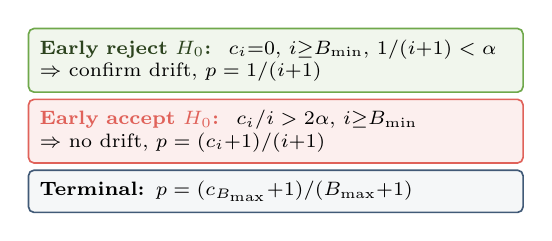
\begin{tikzpicture}[font=\scriptsize,
    box/.style={draw=eaddDeep,line width=0.6pt,rounded corners=2pt,
                fill=white,text width=6.0cm,inner sep=4pt,align=left}]
  \node[box,draw=eaddLime,fill=eaddLime!10] (r) {%
    \textbf{\color{eaddLime!40!black}Early reject $H_0$:}\;
    $c_i{=}0$, $i{\ge}B_{\min}$, $1/(i{+}1)<\alpha$ \\
    $\Rightarrow$ confirm drift, $p=1/(i{+}1)$};
  \node[box,draw=eaddCoral,fill=eaddCoral!10,below=2pt of r] (a) {%
    \textbf{\color{eaddCoral}Early accept $H_0$:}\;
    $c_i/i > 2\alpha$, $i{\ge}B_{\min}$ \\
    $\Rightarrow$ no drift, $p=(c_i{+}1)/(i{+}1)$};
  \node[box,draw=eaddSlate,fill=eaddSlate!5,below=2pt of a] (t) {%
    \textbf{Terminal:} $p=(c_{B_{\max}}{+}1)/(B_{\max}{+}1)$};
\end{tikzpicture}

\column{0.50\textwidth}
\centering
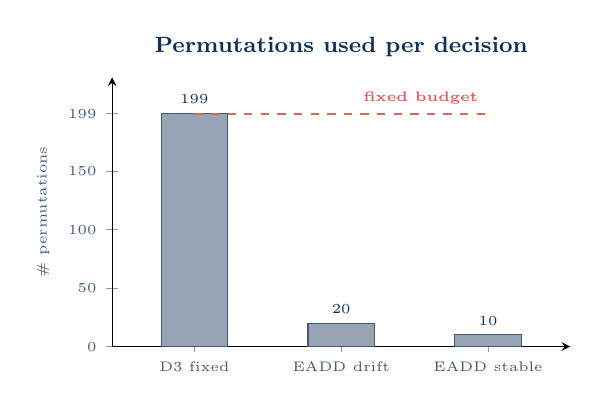
\begin{tikzpicture}[font=\tiny]
  \begin{axis}[
    width=7.4cm,height=5.0cm,
    title={\footnotesize\color{eaddDeep}\textbf{Permutations used per decision}},
    title style={yshift=-2pt},
    ylabel={\#~permutations},
    ymin=0,ymax=230,
    symbolic x coords={D3 fixed,EADD drift,EADD stable},
    xtick=data,
    ytick={0,50,100,150,199},
    ybar,bar width=24pt,
    nodes near coords,
    nodes near coords style={font=\tiny\bfseries,text=eaddDeep},
    axis lines=left,
    xlabel style={font=\tiny,text=eaddSlate},
    ylabel style={font=\tiny,text=eaddSlate},
    every tick label/.style={font=\tiny,text=eaddSlate},
    tick style={eaddSlate!60},
    every axis line/.style={eaddSlate!60},
    enlarge x limits=0.28,
  ]
    \addplot[fill=eaddSlate!55,draw=eaddSlate]
      coordinates {(D3 fixed,199) (EADD drift,20) (EADD stable,10)};
    \draw[eaddCoral,line width=0.7pt,dashed]
      (axis cs:D3 fixed,199) -- (axis cs:EADD stable,199);
    \node[text=eaddCoral,font=\tiny\bfseries,anchor=south east]
      at (axis cs:EADD stable,199) {fixed budget};
  \end{axis}
\end{tikzpicture}

\vspace{0.1em}
\colorbox{eaddTeal!18}{\small\textbf{\color{eaddDeep}90--95\% fewer permutations}
\textbar{} $\alpha$ preserved}
\end{columns}
\end{frame}

% ════════════════════ SHAP + DSI ════════════════════
\begin{frame}{Contribution 2 \textbar{} SHAP Attribution $+$ Drift Severity Index}
\begin{columns}[T,onlytextwidth]
\column{0.48\textwidth}
\textbf{TreeSHAP on the C2ST classifier} (which D3 discards).

\smallskip
\[
\bar\phi_j = \tfrac{1}{n}\sum_i |\phi_j^{(i)}|, \quad
s_j = \bar\phi_j \,/\, \textstyle\sum_k \bar\phi_k
\]
{\scriptsize\color{eaddSlate}Normalised attribution share $\to$ which features drifted.}

\smallskip
\textbf{Drift Severity Index.}
\[
\boxed{\;\mathrm{DSI}=\mathrm{AUC}\times\bigl(1-H_{\mathrm{norm}}(\mathbf{s})\bigr)\;}
\]
{\scriptsize $H_{\mathrm{norm}}(\mathbf{s})=-\sum_j s_j\log_2 s_j \,/\,\log_2 d\in[0,1]$ ---
dimensionality-invariant via $\log_2 d$ normalisation.}

\column{0.52\textwidth}
\centering
\textbf{\small Severity gradient \& prescription tiers}

\vspace{0.3em}
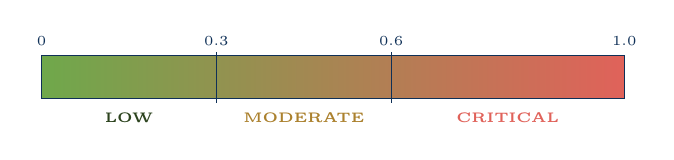
\begin{tikzpicture}[font=\scriptsize]
  \shade[left color=eaddLime,middle color=eaddAmber,right color=eaddCoral]
    (0,0) rectangle (7.4,0.55);
  \draw[eaddDeep,line width=0.4pt] (0,0) rectangle (7.4,0.55);
  \draw[eaddDeep,line width=0.5pt] (2.22,-0.05) -- (2.22,0.60);
  \draw[eaddDeep,line width=0.5pt] (4.44,-0.05) -- (4.44,0.60);
  \node[anchor=north,font=\tiny\bfseries,text=eaddLime!40!black] at (1.11,-0.05) {LOW};
  \node[anchor=north,font=\tiny\bfseries,text=eaddAmber!70!black] at (3.33,-0.05) {MODERATE};
  \node[anchor=north,font=\tiny\bfseries,text=eaddCoral] at (5.92,-0.05) {CRITICAL};
  \node[anchor=south,font=\tiny,text=eaddDeep] at (0,0.55) {0};
  \node[anchor=south,font=\tiny,text=eaddDeep] at (2.22,0.55) {0.3};
  \node[anchor=south,font=\tiny,text=eaddDeep] at (4.44,0.55) {0.6};
  \node[anchor=south,font=\tiny,text=eaddDeep] at (7.4,0.55) {1.0};
\end{tikzpicture}

\vspace{1.2em}
\begin{tabular}{@{}l p{4.6cm}@{}}
\toprule
\textbf{Tier} & \textbf{Recommended action} \\
\midrule
\textcolor{eaddLime!40!black}{\textbf{Low}} ($<\!0.3$)        & Diffuse shift $\to$ scheduled retrain \\
\textcolor{eaddAmber!70!black}{\textbf{Moderate}} (0.3--0.6) & Subset drift $\to$ audit shared source \\
\textcolor{eaddCoral}{\textbf{Critical}} ($>\!0.6$)           & Concentrated $\to$ audit pipeline \\
\bottomrule
\end{tabular}

\vspace{0.3em}
{\scriptsize\itshape\color{eaddSlate}Heuristic tiers; require domain calibration.}
\end{columns}
\end{frame}

% ════════════════════ SECTION 3 ════════════════════
\sectionDivider{03}{Experiments \& Results}

\begin{frame}{Experimental Setup}
\centering
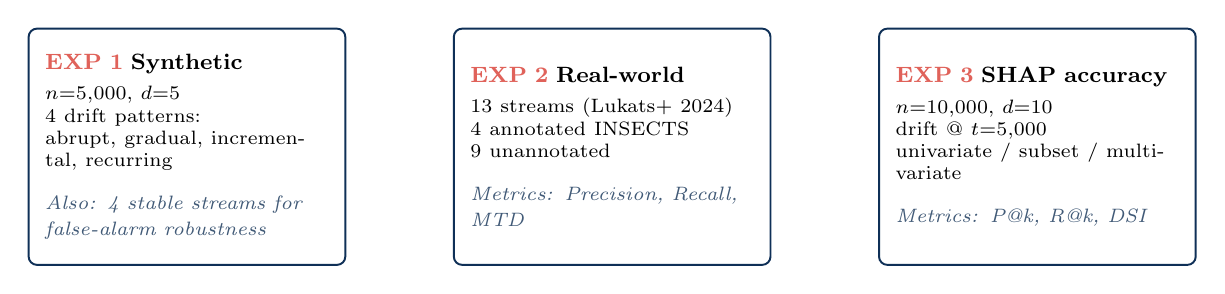
\begin{tikzpicture}[font=\footnotesize,
    card/.style={draw=eaddDeep,line width=0.7pt,rounded corners=3pt,
                 fill=white,minimum width=4.0cm,minimum height=3.0cm,
                 inner sep=6pt,align=left,text width=3.6cm}]
  \node[card] (e1) at (-5.4,0) {
    \textbf{\color{eaddCoral}EXP 1\;}\textbf{Synthetic}\\[3pt]
    \scriptsize $n{=}5{,}000$, $d{=}5$\\
    4 drift patterns:\\
    abrupt, gradual, incremental, recurring\\
    \medskip
    \scriptsize\color{eaddSlate}\textit{Also: 4 stable streams for false-alarm robustness}
  };
  \node[card] (e2) at (0,0) {
    \textbf{\color{eaddCoral}EXP 2\;}\textbf{Real-world}\\[3pt]
    \scriptsize 13 streams (Lukats+ 2024)\\
    4 annotated INSECTS\\
    9 unannotated\\
    \medskip
    \scriptsize\color{eaddSlate}\textit{Metrics: Precision, Recall, MTD}
  };
  \node[card] (e3) at (5.4,0) {
    \textbf{\color{eaddCoral}EXP 3\;}\textbf{SHAP accuracy}\\[3pt]
    \scriptsize $n{=}10{,}000$, $d{=}10$\\
    drift @ $t{=}5{,}000$\\
    univariate / subset / multivariate\\
    \medskip
    \scriptsize\color{eaddSlate}\textit{Metrics: P@k, R@k, DSI}
  };
\end{tikzpicture}

\vspace{0.6em}
\centering
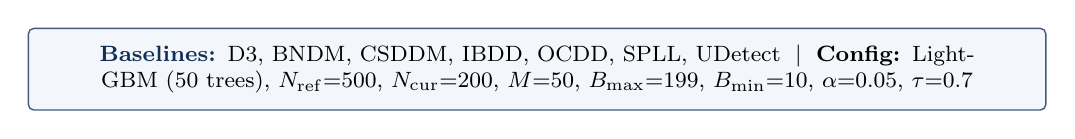
\begin{tikzpicture}[font=\footnotesize]
  \node[draw=eaddSlate,line width=0.5pt,rounded corners=2pt,fill=eaddMist,
        inner sep=6pt,text width=12.5cm,align=center] {
    \textbf{\color{eaddDeep}Baselines:} D3, BNDM, CSDDM, IBDD, OCDD, SPLL, UDetect
    \;\textbar{}\; \textbf{Config:} LightGBM (50 trees),
    $N_\mathrm{ref}{=}500$, $N_\mathrm{cur}{=}200$, $M{=}50$,
    $B_{\max}{=}199$, $B_{\min}{=}10$, $\alpha{=}0.05$, $\tau{=}0.7$};
\end{tikzpicture}
\end{frame}

% ──────────────────── HEADLINE STATS ────────────────────
\begin{frame}{Headline Results}
\vspace{0.5em}
\centering
\statTile{4/4}{synthetic\\coverage}{eaddTeal}\hfill
\statTile{0}{false alarms\\on stable streams}{eaddLime}\hfill
\statTile{8$\boldsymbol{\times}$}{faster MTD\\vs.\ D3 (incremental)}{eaddCoral}\hfill
\statTile{1.00}{P@k$=$R@k\\(univariate SHAP)}{eaddAmber!75!black}

\vspace{1.0em}
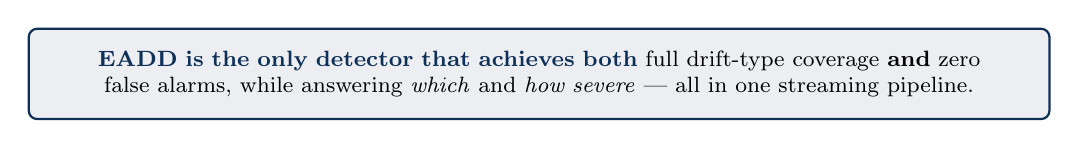
\begin{tikzpicture}[font=\footnotesize]
  \node[draw=eaddDeep,line width=0.8pt,rounded corners=3pt,fill=eaddDeep!8,
        inner sep=8pt,text width=12.4cm,align=center] {%
    \textbf{\color{eaddDeep}EADD is the only detector that achieves both}
    full drift-type coverage \textbf{and} zero false alarms,
    while answering \textit{which} and \textit{how severe} ---
    all in one streaming pipeline.};
\end{tikzpicture}

\vspace{0.6em}
{\scriptsize\color{eaddSlate}Mann--Whitney U vs.\ D3 on autocorrelated streams: $p=0.0101$ ($\tau{=}0.6$).}
\end{frame}

% ──────────────────── RESULT 1: COVERAGE + FA ────────────────────
\begin{frame}{Result 1 \textbar{} Synthetic Coverage vs.\ False Alarms}
\centering
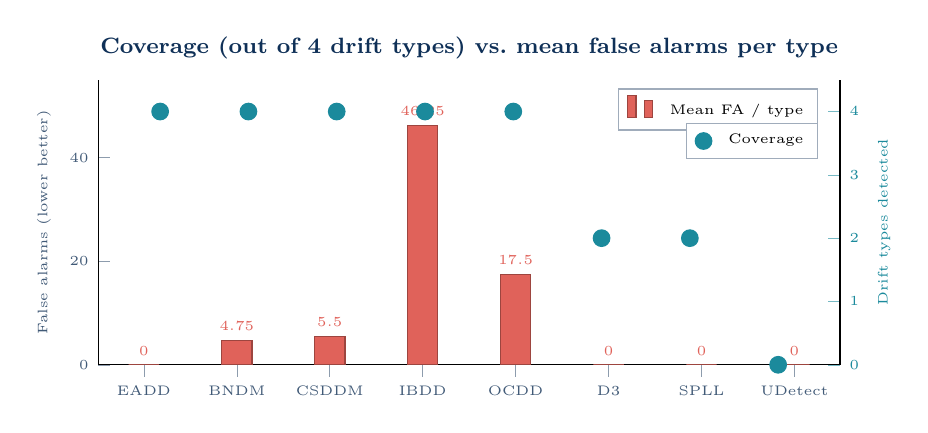
\begin{tikzpicture}[font=\tiny]
  \begin{axis}[
    width=11.0cm,height=5.2cm,
    title={\footnotesize\color{eaddDeep}\textbf{Coverage (out of 4 drift types) vs.\ mean false alarms per type}},
    title style={yshift=-2pt},
    ybar,bar width=11pt,
    ymin=0,ymax=55,
    enlarge x limits=0.07,
    symbolic x coords={EADD,BNDM,CSDDM,IBDD,OCDD,D3,SPLL,UDetect},
    xtick=data,
    ylabel={False alarms (lower better)},
    axis y line*=left,
    axis x line*=bottom,
    every axis label/.style={font=\tiny,text=eaddSlate},
    every tick label/.style={font=\tiny,text=eaddSlate},
    tick style={eaddSlate!60},
    every axis line/.style={eaddSlate!60},
    nodes near coords,
    nodes near coords style={font=\tiny\bfseries,text=eaddCoral},
    nodes near coords align={vertical},
    legend style={at={(0.97,0.97)},anchor=north east,font=\tiny,
                  draw=eaddSlate!50,fill=white,column sep=4pt},
  ]
    \addplot[fill=eaddCoral,draw=eaddCoral!70!black]
      coordinates {(EADD,0.00) (BNDM,4.75) (CSDDM,5.50) (IBDD,46.25)
                   (OCDD,17.50) (D3,0.00) (SPLL,0.00) (UDetect,0)};
    \addlegendentry{Mean FA / type};
  \end{axis}
  % overlay coverage as second axis using markers
  \begin{axis}[
    width=11.0cm,height=5.2cm,
    ymin=0,ymax=4.5,ytick={0,1,2,3,4},
    ylabel={Drift types detected},
    axis y line*=right,
    axis x line=none,
    symbolic x coords={EADD,BNDM,CSDDM,IBDD,OCDD,D3,SPLL,UDetect},
    every axis label/.style={font=\tiny,text=eaddTeal},
    every tick label/.style={font=\tiny,text=eaddTeal},
    tick style={eaddTeal!60},
    every axis line/.style={eaddTeal!60},
    legend style={at={(0.97,0.85)},anchor=north east,font=\tiny,
                  draw=eaddSlate!50,fill=white,column sep=4pt},
  ]
    \addplot[only marks,mark=*,mark size=3pt,eaddTeal]
      coordinates {(EADD,4) (BNDM,4) (CSDDM,4) (IBDD,4)
                   (OCDD,4) (D3,2) (SPLL,2) (UDetect,0)};
    \addlegendentry{Coverage};
  \end{axis}
\end{tikzpicture}

\vspace{0.2em}

\begin{tikzpicture}
\node[fill=eaddTeal,rounded corners=2pt,text=white,font=\footnotesize\bfseries,
      inner sep=5pt,text width=12.0cm,align=center] {%
EADD: \textbf{4/4 coverage} AND \textbf{0 false alarms}.
The other 4/4 detectors (BNDM/CSDDM/IBDD/OCDD) pay heavy FA cost; D3/SPLL hit 0 FA only by missing half the drift types.};
\end{tikzpicture}
\end{frame}

% ──────────────────── RESULT 2: MTD ────────────────────
\begin{frame}{Result 2 \textbar{} INSECTS — Mean Time to Detection}
\centering
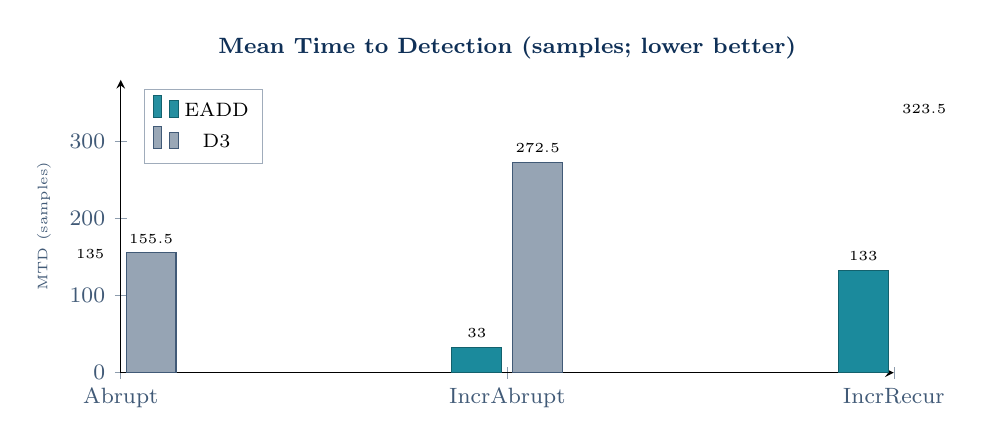
\begin{tikzpicture}[font=\tiny]
  \begin{axis}[
    width=11.4cm,height=5.3cm,
    title={\footnotesize\color{eaddDeep}\textbf{Mean Time to Detection (samples; lower better)}},
    title style={yshift=-2pt},
    ybar=4pt,bar width=18pt,
    ymin=0,ymax=380,
    enlarge x limits=0.25,
    symbolic x coords={Abrupt,IncrAbrupt,IncrRecur},
    xtick=data,
    ylabel={MTD (samples)},
    axis lines=left,
    every axis label/.style={font=\tiny,text=eaddSlate},
    every tick label/.style={font=\footnotesize,text=eaddSlate},
    tick style={eaddSlate!60},
    every axis line/.style={eaddSlate!60},
    nodes near coords,
    nodes near coords style={font=\tiny\bfseries},
    legend style={at={(0.03,0.97)},anchor=north west,legend columns=1,
                  font=\scriptsize,draw=eaddSlate!50,fill=white,fill opacity=0.95,
                  text opacity=1},
  ]
    \addplot[fill=eaddTeal,draw=eaddTeal!70!black]
      coordinates {(Abrupt,135) (IncrAbrupt,33) (IncrRecur,133)};
    \addplot[fill=eaddSlate!55,draw=eaddSlate]
      coordinates {(Abrupt,155.5) (IncrAbrupt,272.5) (IncrRecur,323.5)};
    \legend{EADD,D3}
  \end{axis}
\end{tikzpicture}

\vspace{0.2em}
\centering
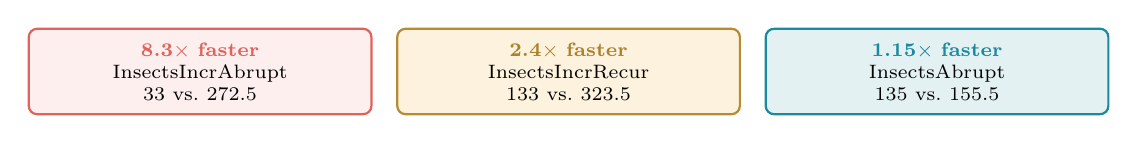
\begin{tikzpicture}[font=\scriptsize]
  \node[draw=eaddCoral,line width=0.8pt,rounded corners=3pt,fill=eaddCoral!10,
        inner sep=5pt,text width=4.0cm,align=center] (a) {%
    \textbf{\color{eaddCoral}8.3$\times$ faster}\\InsectsIncrAbrupt\\\scriptsize 33 vs.\ 272.5};
  \node[draw=eaddAmber!75!black,line width=0.8pt,rounded corners=3pt,fill=eaddAmber!18,
        inner sep=5pt,text width=4.0cm,align=center,right=0.3cm of a] (b) {%
    \textbf{\color{eaddAmber!70!black}2.4$\times$ faster}\\InsectsIncrRecur\\\scriptsize 133 vs.\ 323.5};
  \node[draw=eaddTeal,line width=0.8pt,rounded corners=3pt,fill=eaddTeal!12,
        inner sep=5pt,text width=4.0cm,align=center,right=0.3cm of b] (c) {%
    \textbf{\color{eaddTeal}1.15$\times$ faster}\\InsectsAbrupt\\\scriptsize 135 vs.\ 155.5};
\end{tikzpicture}

\vspace{0.3em}
{\scriptsize\color{eaddSlate}\itshape EADD beats D3 on MTD in all three jointly detected INSECTS streams; InsectsGradual missed by both.}
\end{frame}

% ──────────────────── RESULT 3: SHAP ATTRIBUTION ────────────────────
\begin{frame}{Result 3 \textbar{} SHAP Attribution Accuracy}
\begin{columns}[T,onlytextwidth]
\column{0.55\textwidth}
\centering
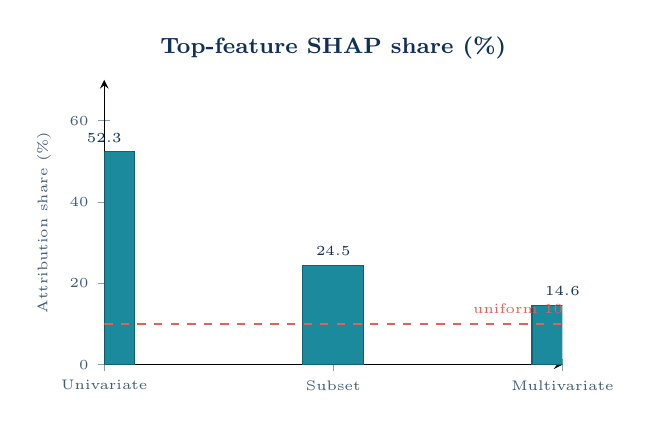
\begin{tikzpicture}[font=\tiny]
  \begin{axis}[
    width=7.4cm,height=5.2cm,
    title={\footnotesize\color{eaddDeep}\textbf{Top-feature SHAP share (\%)}},
    title style={yshift=-2pt},
    ybar,bar width=22pt,
    ymin=0,ymax=70,
    enlarge x limits=0.22,
    symbolic x coords={Univariate,Subset,Multivariate},
    xtick=data,
    ylabel={Attribution share (\%)},
    axis lines=left,
    every axis label/.style={font=\tiny,text=eaddSlate},
    every tick label/.style={font=\tiny,text=eaddSlate},
    tick style={eaddSlate!60},
    every axis line/.style={eaddSlate!60},
    nodes near coords,
    nodes near coords style={font=\tiny\bfseries,text=eaddDeep},
  ]
    \addplot[fill=eaddTeal,draw=eaddTeal!70!black]
      coordinates {(Univariate,52.3) (Subset,24.5) (Multivariate,14.6)};
    \draw[eaddCoral,dashed,line width=0.6pt]
      (axis cs:Univariate,10) -- (axis cs:Multivariate,10)
      node[pos=0.92,above,font=\tiny,text=eaddCoral] {uniform $10\%$};
  \end{axis}
\end{tikzpicture}

\column{0.45\textwidth}
\centering
\textbf{\small Perfect attribution \textbar{} P@k $=$ R@k $=$ 1.0}

\vspace{0.3em}
\setlength{\tabcolsep}{4pt}
\begin{tabular}{@{}l c c c@{}}
\toprule
\textbf{Scenario} & \textbf{AUC} & \textbf{Top feat.} & \textbf{DSI} \\
\midrule
Univariate (1/10)    & 0.784 & \textbf{F3} (52.3\%) & 0.193 \\
Subset (3/10)        & 0.809 & F5 (24.5\%)          & 0.096 \\
Multivariate (10/10) & 0.806 & F2 (14.6\%)          & 0.016 \\
\bottomrule
\end{tabular}

\vspace{0.5em}
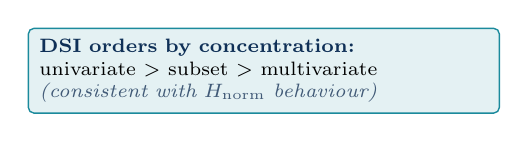
\begin{tikzpicture}[font=\scriptsize]
\node[fill=eaddTeal!12,draw=eaddTeal,line width=0.5pt,rounded corners=2pt,
      inner sep=4pt,text width=5.7cm,align=left] {%
\textbf{\color{eaddDeep}DSI orders by concentration:}\\
univariate $>$ subset $>$ multivariate\\
\scriptsize\color{eaddSlate}\textit{(consistent with $H_{\mathrm{norm}}$ behaviour)}};
\end{tikzpicture}
\end{columns}
\end{frame}

% ──────────────────── RESULT 4: FALSE ALARM ROBUSTNESS ────────────────────
\begin{frame}{Result 4 \textbar{} False-Alarm Robustness on Stable Streams}
\centering
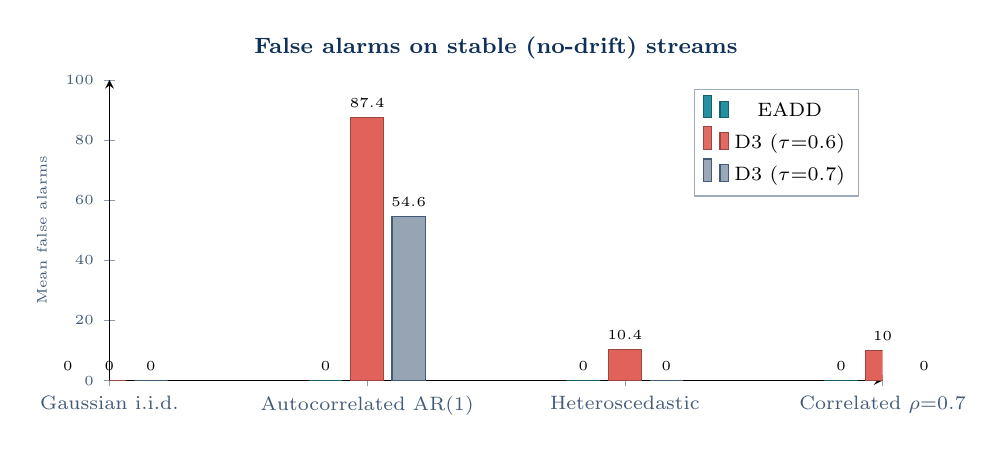
\begin{tikzpicture}[font=\tiny]
  \begin{axis}[
    width=11.4cm,height=5.4cm,
    title={\footnotesize\color{eaddDeep}\textbf{False alarms on stable (no-drift) streams}},
    title style={yshift=-2pt},
    ybar=3pt,bar width=12pt,
    ymin=0,ymax=100,
    enlarge x limits=0.20,
    symbolic x coords={Gaussian i.i.d.,Autocorrelated AR(1),Heteroscedastic,{Correlated $\rho{=}0.7$}},
    xtick=data,
    xticklabel style={font=\scriptsize,text=eaddSlate,align=center},
    ylabel={Mean false alarms},
    axis lines=left,
    every axis label/.style={font=\tiny,text=eaddSlate},
    every tick label/.style={font=\tiny,text=eaddSlate},
    tick style={eaddSlate!60},
    every axis line/.style={eaddSlate!60},
    nodes near coords,
    nodes near coords style={font=\tiny\bfseries},
    legend style={at={(0.97,0.97)},anchor=north east,legend columns=1,
                  font=\scriptsize,draw=eaddSlate!50,fill=white,fill opacity=0.95,
                  text opacity=1},
  ]
    \addplot[fill=eaddTeal,draw=eaddTeal!70!black]
      coordinates {(Gaussian i.i.d.,0) (Autocorrelated AR(1),0) (Heteroscedastic,0) ({Correlated $\rho{=}0.7$},0)};
    \addplot[fill=eaddCoral,draw=eaddCoral!70!black]
      coordinates {(Gaussian i.i.d.,0) (Autocorrelated AR(1),87.4) (Heteroscedastic,10.4) ({Correlated $\rho{=}0.7$},10.0)};
    \addplot[fill=eaddSlate!55,draw=eaddSlate]
      coordinates {(Gaussian i.i.d.,0) (Autocorrelated AR(1),54.6) (Heteroscedastic,0) ({Correlated $\rho{=}0.7$},0)};
    \legend{EADD,D3 ($\tau{=}0.6$),D3 ($\tau{=}0.7$)}
  \end{axis}
\end{tikzpicture}

\vspace{0.2em}
\centering
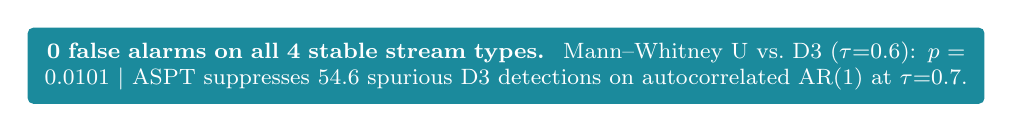
\begin{tikzpicture}[font=\footnotesize]
  \node[fill=eaddTeal,rounded corners=2pt,text=white,inner sep=5pt,
        text width=11.8cm,align=center] {%
    \textbf{0 false alarms on all 4 stable stream types.}\;
    Mann--Whitney U vs.\ D3 ($\tau{=}0.6$): \textbf{$p=0.0101$} \textbar{}
    ASPT suppresses 54.6 spurious D3 detections on autocorrelated AR(1) at $\tau{=}0.7$.};
\end{tikzpicture}
\end{frame}

% ════════════════════ SECTION 4 ════════════════════
\sectionDivider{04}{Ablation \& Cost}

\begin{frame}{Ablation \textbar{} Where Does the Gain Come From?}
\begin{columns}[T,onlytextwidth]
\column{0.56\textwidth}
\centering
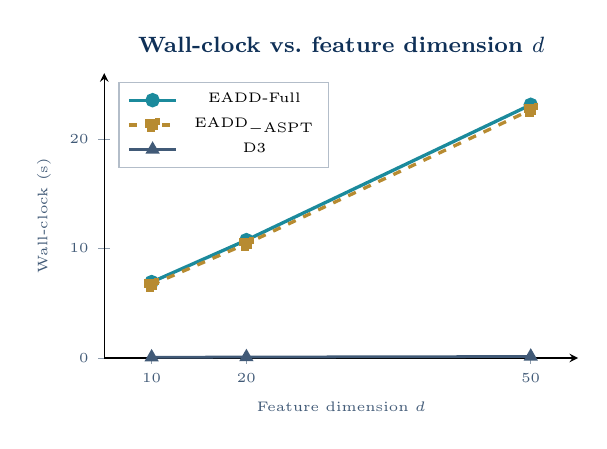
\begin{tikzpicture}[font=\tiny]
  \begin{axis}[
    width=7.6cm,height=5.2cm,
    title={\footnotesize\color{eaddDeep}\textbf{Wall-clock vs.\ feature dimension $d$}},
    title style={yshift=-2pt},
    xlabel={Feature dimension $d$},
    ylabel={Wall-clock (s)},
    xmin=5,xmax=55,ymin=0,ymax=26,
    xtick={10,20,50},
    axis lines=left,
    every axis label/.style={font=\tiny,text=eaddSlate},
    every tick label/.style={font=\tiny,text=eaddSlate},
    tick style={eaddSlate!60},
    every axis line/.style={eaddSlate!60},
    legend style={at={(0.03,0.97)},anchor=north west,font=\tiny,
                  draw=eaddSlate!40,fill=white,column sep=4pt},
    mark size=2pt,
  ]
    \addplot[eaddTeal,line width=1.2pt,mark=*]
      coordinates {(10,6.93) (20,10.76) (50,23.11)};
    \addplot[eaddAmber!75!black,line width=1.2pt,mark=square*,dashed]
      coordinates {(10,6.68) (20,10.43) (50,22.64)};
    \addplot[eaddSlate,line width=1.0pt,mark=triangle*]
      coordinates {(10,0.07) (20,0.09) (50,0.14)};
    \legend{EADD-Full,EADD$_{-\mathrm{ASPT}}$,D3}
  \end{axis}
\end{tikzpicture}

\column{0.44\textwidth}
\textbf{Decomposing the gain}

\smallskip
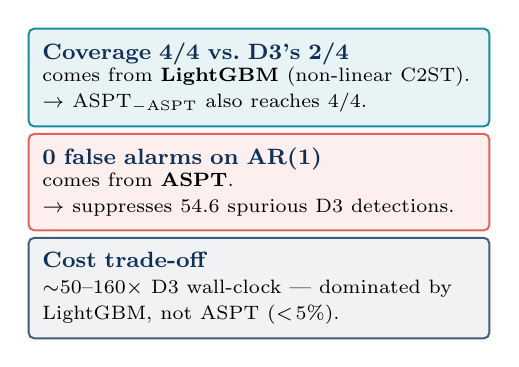
\begin{tikzpicture}[font=\footnotesize,
  card/.style={draw,line width=0.7pt,rounded corners=2pt,
               text width=5.5cm,align=left,inner sep=5pt}]
  \node[card,draw=eaddTeal,fill=eaddTeal!10] (a) {%
    \textbf{\color{eaddDeep}Coverage 4/4 vs.\ D3's 2/4}\\
    \scriptsize comes from \textbf{LightGBM} (non-linear C2ST).\\
    \scriptsize $\to$ ASPT$_{-\mathrm{ASPT}}$ also reaches 4/4.};
  \node[card,draw=eaddCoral,fill=eaddCoral!10,below=2pt of a] (b) {%
    \textbf{\color{eaddDeep}0 false alarms on AR(1)}\\
    \scriptsize comes from \textbf{ASPT}.\\
    \scriptsize $\to$ suppresses 54.6 spurious D3 detections.};
  \node[card,draw=eaddSlate,fill=eaddSlate!8,below=2pt of b] (c) {%
    \textbf{\color{eaddDeep}Cost trade-off}\\
    \scriptsize $\sim$50--160$\times$ D3 wall-clock --- dominated by LightGBM, not ASPT ($<\!5\%$).};
\end{tikzpicture}
\end{columns}
\end{frame}

% ════════════════════ SECTION 5 ════════════════════
\sectionDivider{05}{Limits \& Outlook}

\begin{frame}{Limitations \& Future Work}
\begin{columns}[T,onlytextwidth]
\column{0.50\textwidth}
\textbf{\color{eaddCoral}Limitations}
\begin{itemize}\setlength\itemsep{2pt}\footnotesize
  \item Wall-clock $\sim$50--160$\times$ D3 --- LightGBM retrains every $M{=}50$ steps.
  \item \textbf{Multiple testing over time:} $\sim$600 tests / 30K samples;
        Bonferroni $\alpha'{\approx}8.3{\times}10^{-5}$ below ASPT's $1/(B_{\max}{+}1){=}0.005$ floor.\\
        \scriptsize\itshape Zero-FA result empirical, not theoretically guaranteed.
  \item DSI tier boundaries heuristic; never triggered above LOW in experiments.
  \item SHAP attributions correlational, not causal.
  \item No isolation of reservoir sampling vs.\ window config contributions.
\end{itemize}

\column{0.50\textwidth}
\textbf{\color{eaddTeal}Future Work}
\begin{itemize}\setlength\itemsep{2pt}\footnotesize
  \item Anytime-valid \textbf{e-values} for streaming FWER control.
  \item \textbf{Causal} attribution (Budhathoki+ AISTATS 2021).
  \item Multi-domain \textbf{DSI calibration} to ground tier boundaries empirically.
  \item Adversarial robustness of discriminative drift detectors.
  \item Per-feature operating curves under correlation $\to$ feature-group SHAP.
\end{itemize}

\vspace{0.5em}

\begin{tikzpicture}[font=\scriptsize]
  \node[fill=eaddDeep,rounded corners=2pt,text=white,inner sep=5pt,
        text width=6.2cm,align=center,font=\scriptsize] {%
    \textbf{Open invitation.} EADD is a starting point ---
    each gap above is a separate research thread.};
\end{tikzpicture}
\end{columns}
\end{frame}

% ════════════════════ CONCLUSION ════════════════════
\begin{frame}{Conclusion}
\vspace{0.3em}
\centering

\begin{tikzpicture}[font=\footnotesize,
    pill/.style={fill=eaddDeep,text=white,rounded corners=10pt,
                 inner xsep=10pt,inner ysep=5pt,font=\bfseries}]
  \node[pill] {EADD answers \textcolor{eaddAmber}{WHETHER},
               \textcolor{eaddAmber}{WHEN},
               \textcolor{eaddAmber}{WHICH}, and
               \textcolor{eaddAmber}{HOW SEVERE} --- in one pipeline.};
\end{tikzpicture}

\vspace{0.8em}
\centering
\statTile{4/4}{coverage}{eaddTeal}\hfill
\statTile{0}{false alarms}{eaddLime}\hfill
\statTile{8$\boldsymbol{\times}$}{faster MTD}{eaddCoral}\hfill
\statTile{1.00}{SHAP P@k}{eaddAmber!75!black}

\vspace{0.8em}
\begin{columns}[T,onlytextwidth]
\column{0.50\textwidth}
\textbf{\color{eaddDeep}What we built}
\begin{itemize}\setlength\itemsep{1pt}\footnotesize
  \item ASPT $+$ $H_{\mathrm{pred}}$ --- rigorous confirmation, 90--95\% perm savings.
  \item SHAP $+$ DSI --- feature-level diagnosis $+$ severity.
  \item Benchmark vs.\ 7 unsupervised detectors.
\end{itemize}

\column{0.50\textwidth}
\textbf{\color{eaddDeep}What it gives MLOps}
\begin{itemize}\setlength\itemsep{1pt}\footnotesize
  \item Reliable alarms on autocorrelated production streams.
  \item Actionable diagnoses, not just binary flags.
  \item Severity-tiered prescriptions for response.
\end{itemize}
\end{columns}
\end{frame}

% ════════════════════ THANK YOU ════════════════════
\begin{frame}[plain,noframenumbering]

\begin{tikzpicture}[remember picture,overlay]
  \fill[eaddDeep] (current page.south west) rectangle (current page.north east);
  \fill[eaddTeal,opacity=0.45]
    (current page.south east) -- ([xshift=-8cm]current page.south east)
    -- ([xshift=-4cm]current page.north east) -- (current page.north east) -- cycle;
  \foreach \i in {0,1,2,3,4}{
    \fill[eaddAmber,opacity={0.05+0.02*\i}]
      ([xshift=2cm+0.4*\i cm,yshift=2cm+0.3*\i cm]current page.south west)
      circle ({1.0cm+0.4*\i cm});
  }
  \node[anchor=center,text=white,font=\fontsize{56}{60}\bfseries]
    at ([yshift=0.8cm]current page.center) {Thank You.};
  \node[anchor=center,text=eaddAmber,font=\Large\itshape]
    at ([yshift=-0.5cm]current page.center) {Questions \& discussion welcome.};
  \node[anchor=center,text=white,font=\small]
    at ([yshift=-1.8cm]current page.center)
    {\textbf{Nusrat Begum} \textbar{} \texttt{nusrat.beg@student.mahidol.ac.th}};
  \node[anchor=south,text=white!60,font=\scriptsize]
    at ([yshift=0.6cm]current page.south) {Code + paper available at the project repository.};
\end{tikzpicture}
\end{frame}

% ════════════════════ APPENDIX ════════════════════
\appendix

\begin{frame}{Backup \textbar{} Runtime Scaling --- Window $N_\mathrm{cur}$}
\begin{columns}[T,onlytextwidth]
\column{0.55\textwidth}
\centering
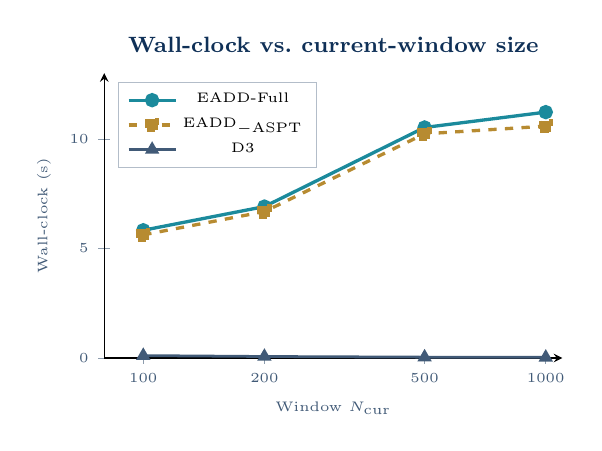
\begin{tikzpicture}[font=\tiny]
  \begin{axis}[
    width=7.4cm,height=5.2cm,
    title={\footnotesize\color{eaddDeep}\textbf{Wall-clock vs.\ current-window size}},
    title style={yshift=-2pt},
    xlabel={Window $N_\mathrm{cur}$},
    ylabel={Wall-clock (s)},
    xmin=80,xmax=1100,ymin=0,ymax=13,
    xmode=log,log basis x=10,
    xtick={100,200,500,1000},
    xticklabels={100,200,500,1000},
    axis lines=left,
    every axis label/.style={font=\tiny,text=eaddSlate},
    every tick label/.style={font=\tiny,text=eaddSlate},
    tick style={eaddSlate!60},
    every axis line/.style={eaddSlate!60},
    legend style={at={(0.03,0.97)},anchor=north west,font=\tiny,
                  draw=eaddSlate!40,fill=white},
    mark size=2pt,
  ]
    \addplot[eaddTeal,line width=1.2pt,mark=*]
      coordinates {(100,5.83) (200,6.91) (500,10.52) (1000,11.22)};
    \addplot[eaddAmber!75!black,line width=1.2pt,mark=square*,dashed]
      coordinates {(100,5.62) (200,6.68) (500,10.23) (1000,10.58)};
    \addplot[eaddSlate,line width=1.0pt,mark=triangle*]
      coordinates {(100,0.11) (200,0.07) (500,0.04) (1000,0.03)};
    \legend{EADD-Full,EADD$_{-\mathrm{ASPT}}$,D3}
  \end{axis}
\end{tikzpicture}

\column{0.45\textwidth}
\vspace{0.4em}
\begin{itemize}\footnotesize
  \item $N_\mathrm{cur}{=}200{\to}1000$: EADD time grows only \textbf{1.6$\times$}.
  \item LightGBM cost sub-linear in $N$, near-linear in $d$.
  \item ASPT overhead $<\!5\%$ across window sizes.
\end{itemize}

\vspace{0.5em}
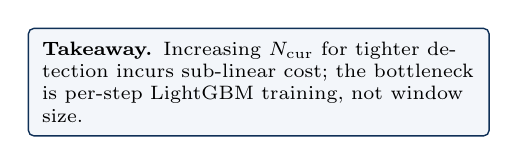
\begin{tikzpicture}[font=\footnotesize]
  \node[fill=eaddMist,draw=eaddDeep,line width=0.5pt,rounded corners=2pt,
        inner sep=5pt,text width=5.5cm,align=left,font=\scriptsize] {%
    \textbf{Takeaway.} Increasing $N_\mathrm{cur}$ for tighter detection
    incurs sub-linear cost; the bottleneck is per-step LightGBM training, not window size.};
\end{tikzpicture}
\end{columns}
\end{frame}

\begin{frame}{Backup \textbar{} Correlated Features ($d{=}10$)}
\centering
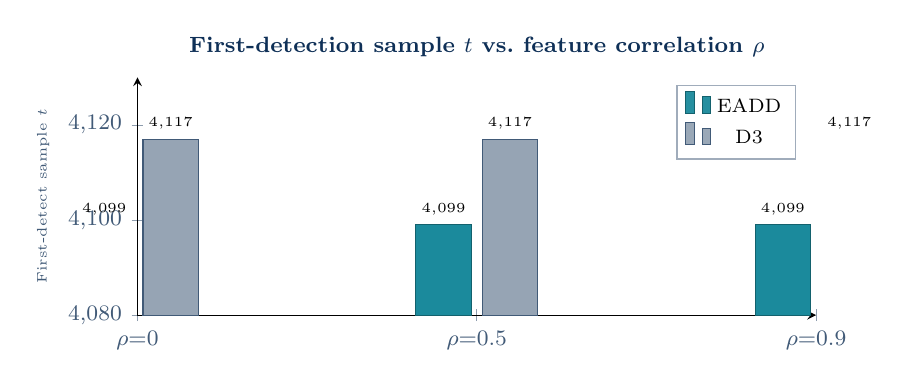
\begin{tikzpicture}[font=\tiny]
  \begin{axis}[
    width=10.2cm,height=4.6cm,
    title={\footnotesize\color{eaddDeep}\textbf{First-detection sample $t$ vs.\ feature correlation $\rho$}},
    title style={yshift=-2pt},
    ybar=4pt,bar width=20pt,
    ymin=4080,ymax=4130,
    enlarge x limits=0.25,
    symbolic x coords={$\rho{=}0$,$\rho{=}0.5$,$\rho{=}0.9$},
    xtick=data,
    ylabel={First-detect sample $t$},
    axis lines=left,
    every axis label/.style={font=\tiny,text=eaddSlate},
    every tick label/.style={font=\footnotesize,text=eaddSlate},
    tick style={eaddSlate!60},
    every axis line/.style={eaddSlate!60},
    nodes near coords,
    nodes near coords style={font=\tiny\bfseries},
    legend style={at={(0.97,0.97)},anchor=north east,legend columns=1,
                  font=\scriptsize,draw=eaddSlate!50,fill=white,fill opacity=0.95,
                  text opacity=1},
  ]
    \addplot[fill=eaddTeal,draw=eaddTeal!70!black]
      coordinates {($\rho{=}0$,4099) ($\rho{=}0.5$,4099) ($\rho{=}0.9$,4099)};
    \addplot[fill=eaddSlate!55,draw=eaddSlate]
      coordinates {($\rho{=}0$,4117) ($\rho{=}0.5$,4117) ($\rho{=}0.9$,4117)};
    \legend{EADD,D3}
  \end{axis}
\end{tikzpicture}

\vspace{0.3em}
\begin{itemize}\footnotesize
  \item Cholesky-mixed Gaussian; $+2\sigma$ shift in 3 features at $t{=}4000$.
  \item EADD detection robust to correlation; stable correlated streams give \textbf{0 FA}.
  \item SHAP under correlation $\to$ interpret at \textbf{feature-group} granularity.
\end{itemize}
\end{frame}

\end{document}
